\documentclass[12pt,letterpaper]{article}
\usepackage[margin=1in]{geometry}
\usepackage{chngpage}
\usepackage[english]{babel}
\usepackage[utf8x]{inputenc}
\usepackage{amsmath}
\usepackage{amssymb} 
% \usepackage[retainorgcmds]{IEEEtrantools}
\usepackage{graphicx}
\usepackage{tabularx}
\usepackage{kpfonts}    % for nice fonts
\usepackage{microtype} 
\usepackage{booktabs}   % for nice tables
\usepackage{bm}         % for bold math
\usepackage{listings}   % for inserting code
\usepackage{verbatim}   % useful for program listings
\usepackage{color}  
\usepackage[colorlinks=true]{hyperref}
% use for hypertext
\hypersetup{
	colorlinks=false,       % false: boxed links; true: colored links
	linkcolor=green,        % color of internal links
	citecolor=blue,        % color of links to bibliography
	filecolor=magenta,     % color of file links
	urlcolor=blue         
}
\usepackage[colorinlistoftodos]{todonotes}
\usepackage{natbib}
\usepackage{float}
\usepackage{adjustbox}
\usepackage[capitalise]{cleveref}
\usepackage{xcolor}

\usepackage{longtable,threeparttablex}
\usepackage{subcaption}



%++++++++++++++++++++++++++++++++++++++++


\begin{document}

\begin{center}
\large IEMS-469 Dynamic Programming  HW2

\bigskip
Weijia Zhao \footnote{Weijia.Zhao@kellogg.northwestern.edu}\\
Kellogg Finance

\bigskip
This version: \today
\end{center}

\newpage
Outline: Due to the difficulties to access Deepdish computing resources (too crowded) and the fact that I cannot move files using either Cyberduck/FileZilla (says I am not authorized to do so), I use Northwestern Quest for the the training of question (b) Pong-v0 in this homework assignment. (I have an existing type I account and the GPU used for this homework is A100). (You can also find a copy on Google Colab \href{https://colab.research.google.com/drive/1P2JLPoPdEyRfwSj1ebTzGk2u2wVtkD0G?usp=sharing}{HERE}). Question (a) is fairly easy and the computation is extremely fast even just using CPU.\\

I use a moving average with a constant decay rate to calculate the average reward versus training epochs rather than only consider the most recent 10 epochs or so as
\begin{itemize}
\item (1) Moving average technically takes into account all historical episodes and is less random than the average of 10 most recent epochs (eg: when you just get 10 consecutive good results by luck)
\item (2) Moving average can be easily implemented iteratively along with the training process with lower computational effort: $MA_t=(1-\alpha)MA_{t-1}+\alpha R_t$
\end{itemize}

The network structure used for each problem is:
\begin{itemize}
\item (Cartpole): Fully connected$\rightarrow$Relu$\rightarrow$Fully connected$\rightarrow$Softmax
\item (Pong): Following what you showed in TA session, I first stack four steps of graphs (i.e. four input channels) together as each individual block. Then Convolution with kernel 5 stride 2 output channel 16$\rightarrow$Batch Normalization$\rightarrow$Relu$\rightarrow$ Convolution with kernel 5 stride 2 output channel 32$\rightarrow$Batch Normalization$\rightarrow$Relu$\rightarrow$Convolution with kernel 5 stride 2 output channel 32$\rightarrow$Batch Normalization$\rightarrow$Relu$\rightarrow$Fully connected$\rightarrow$Relu$\rightarrow$Fully Connected (output dim=2 for action network or output dim=1 for state value network)$\rightarrow$Softmax (only for action network)
\end{itemize}

\section{Cartpole}
As mentioned, this model is trained with CPU due to its simplicity. A base also seems unnecessary (also the hw seems only require a base for Q2) since a model without a base can converge to optimal within 500 epochs. I do provide a file with base in "junk/1\_cartpole\_base.py" along with its output "junk/1\_cartpole.txt" in case you are looking for it, apparently the pattern that adding a base slows down the convergence is not universal and it is likely related to the fact that I reduce the learning rate to accommodate much larger loss (likely also larger derivatives) after adding value losses. Nevertheless, I did not try to optimize the hyperparameter in this questions as it converges within 1 or several minutes even in the worst case scenario. Using a base here does not improve the volatility much either since the output without a baselien is already pretty good.\\

The plot of individual epoch reward is given in the following graph: as expected, policy gradient method is quite volatile (with base generate a almost identical output). My initial value for the moving average smoother is 10. Also I would like to mention that even after reaching the best, there is still the possibility that reward goes down or fluctuate following some particular episodes and then recover later (i.e. the convergence is stochastic rather than deterministic). 
 \begin{figure}[H]
 	\centering
 	\caption{Cartpole game}
 	\begin{subfigure}[h]{0.9\textwidth}
 		\centering
 		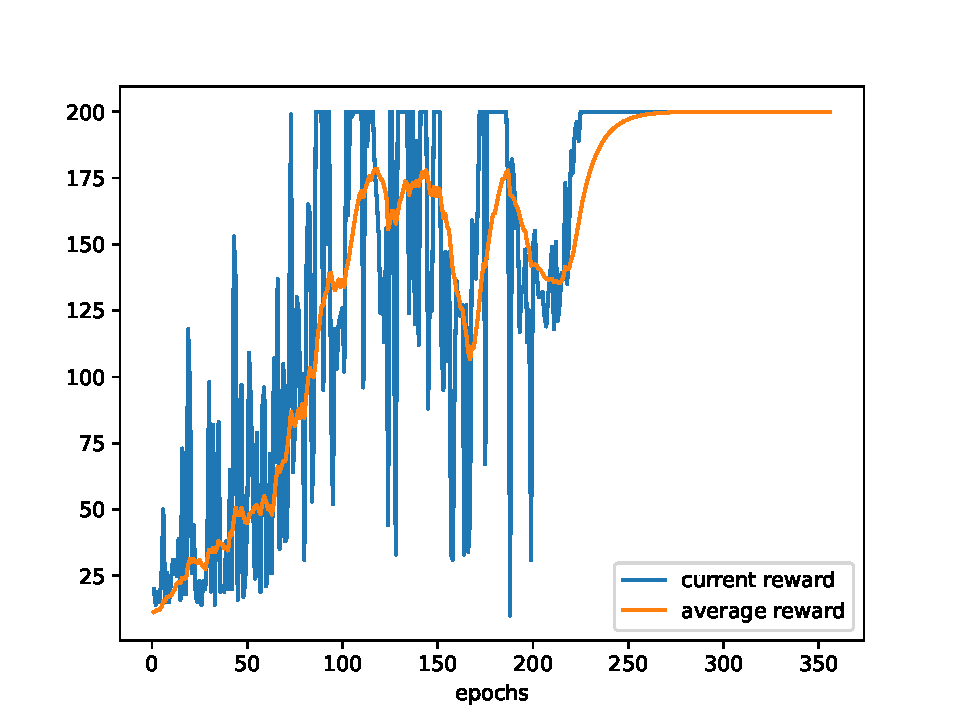
\includegraphics[width=\textwidth]{/Users/lesliezhao/Dropbox/nu_course/2021_fall/DP/IEMS469_HW_LWZ/hw2/1_cartpole.pdf}
 		\caption{Policy Gradient}
 	\end{subfigure}
 \end{figure}


\section{Pong}
As mentioned, I train the model with Northwestern Quest due to inaccessibility of Deepdish (You can also find a copy on Google Colab \href{https://colab.research.google.com/drive/1P2JLPoPdEyRfwSj1ebTzGk2u2wVtkD0G?usp=sharing}{HERE}). I use a relatively small learning rate 1e-5 after some trials (as I consulted you the last Friday, even a learning rate 1e-3 seems to be too large with a convolutional layer and it quickly goes to boundary and loss stays at 0 after that). I stopped the training after 5000 epochs (maybe there is still chance for improving the performance since i am using a relatively powerful NN structure, but I decided to stop it anyway) in about 9 hours, somehow this is slower than I originally expected. Also seems to me the program is relatively faster at the beginning and then as the model improves, each epoch takes much longer time. My explanation is that my agent plays badly at the beginning so it quickly lose the game but later the agent's skill improves and it take much longer time to reach a win/loss between my agent and the computer's agent. (Please let me know if there are any other reasons). Overall the model is learning since the average score increases over time. My initial value for the moving average smoother is 10.

The first time a current reward is greater than 0 is episode 1750. The first time a running reward is greater than 0 is episode 2732. Seems to me the improvement of performance slows down after 4000 epochs though it still possible that here is just a saddle point/local optimal and the model will eventually cross it and improve again later. 
 \begin{figure}[H]
	\centering
	\caption{Pong game}
	\begin{subfigure}[h]{0.9\textwidth}
		\centering
		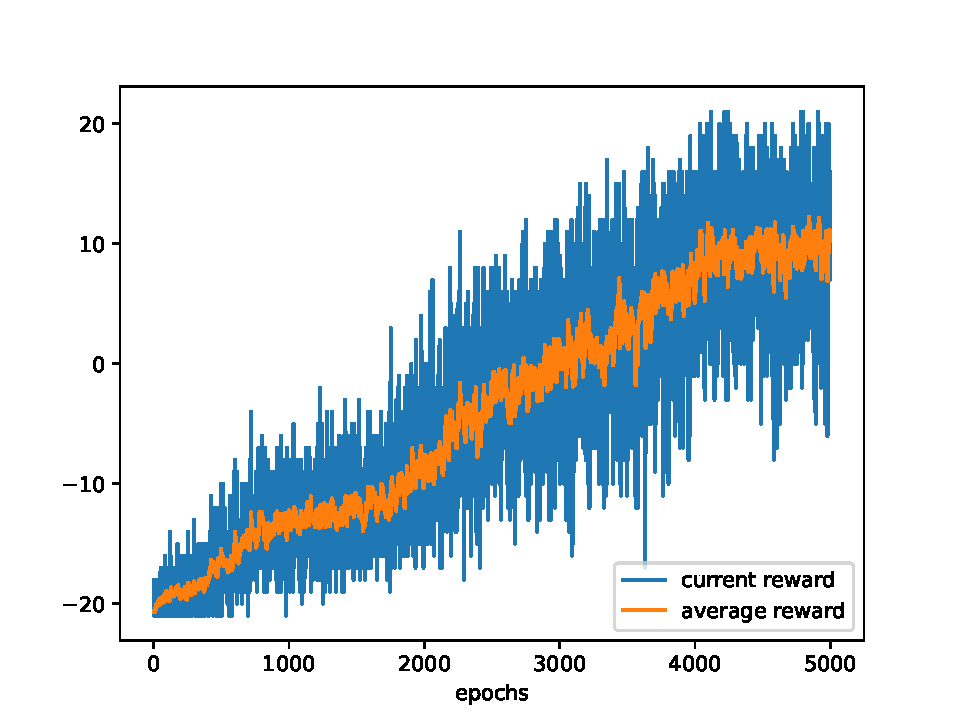
\includegraphics[width=\textwidth]{/Users/lesliezhao/Dropbox/nu_course/2021_fall/DP/IEMS469_HW_LWZ/hw2/2_pong.pdf}
		\caption{Policy Gradient}
	\end{subfigure}
\end{figure}



\end{document}
